\documentclass[12pt]{article}

\usepackage[margin=1in]{geometry}
\usepackage{amsmath,amssymb}
\usepackage{booktabs}
\usepackage{graphicx}
\usepackage{setspace}
\usepackage{caption}
\usepackage[hidelinks]{hyperref}
\usepackage{natbib}
\usepackage{threeparttable}
\usepackage{float}

\graphicspath{{../figures/}{figures/}}
\onehalfspacing
\captionsetup{font=small,labelfont=bf}

% Rupee symbol: portable definition (works under pdflatex without extra fonts)
\newcommand{\rupee}{\text{Rs.}\,}

\title{\textbf{Regulating the Retail Options Boom:\\
Evidence from India's 2024--25 Equity Index Derivatives Reforms}\thanks{%
We thank the Securities and Exchange Board of India (SEBI) for making the
underlying market statistics publicly available. All data used in this paper
are public and aggregate; sources and replication details appear in
Appendix~\ref{app:data}. All errors are our own.
\emph{AI-use disclosure (SSRN policy):} in preparing this paper the authors
used a large language model (Claude, Anthropic) to assist with data-extraction
code, statistical programming, and drafting. All data, analyses, results, and
conclusions were specified, reviewed, and verified by the authors, who take
full responsibility for the content of this paper.}}

\author{Anklesh Rawat\thanks{Independent researcher. Email:
\texttt{ankleshrawat5@duck.com}. Corresponding author.}
\and Shreshtha Rawat\thanks{Independent researcher.}}

\date{This version: July 2026}

\begin{document}

\maketitle

\begin{abstract}
\noindent Between October 2024 and April 2025 the Securities and Exchange
Board of India (SEBI) rolled out the most aggressive package of retail
derivatives curbs attempted in a major market: a package spanning
weekly-expiry rationalization, a threefold increase in minimum contract
size, and tighter margining and position monitoring. We assemble a 48-month panel of exchange-level turnover
(April 2022--March 2026, NSE and BSE combined) from SEBI Monthly Bulletin
annexure tables and combine it with cohort-level participation data from
SEBI's own studies to provide early causal evidence on the reforms. Using
stock options---untargeted by the reforms---as a within-market control, a
trend-adjusted difference-in-differences design implies that index-options
notional turnover fell 37--43\% below its counterfactual path in the six
months following the first wave, while premium turnover fell far less
(\(-\)13\% year on year), consistent with a compositional shift away from
deep out-of-the-money weekly contracts. Participation effects were large and
fell hardest on the smallest traders, the mechanical incidence of a minimum
contract size: unique traders fell 20\% year on year, with declines of
25--36 log points concentrated in the smallest turnover cohorts
(difference-in-differences estimate \(-\)47 log points, permutation-robust).
We find no evidence of substitution into the cash market, which contracted
alongside; substitution into products outside our panel cannot be ruled out.
Aggregate turnover effects attenuate by FY2026 as activity migrated across
exchanges, adapted to larger contracts, and---from January 2026---faced a
rule-driven downward recalibration of lot sizes; participation effects
persist through the latest available data.\\[6pt]
\textbf{Keywords:} derivatives regulation; retail investors; index options;
SEBI; difference-in-differences; market microstructure; India\\
\textbf{JEL codes:} G14, G18, G28, G12, G41
\end{abstract}

\newpage

\section{Introduction}\label{sec:intro}

India's equity index options market grew from a sideshow into the largest
derivatives market in the world by contract volume in less than five years.
Average daily premium turnover (the rupee amount paid for options, as
distinct from the notional value of the underlying exposure) in index
options rose at a compound annual rate
of 72\% between FY2020 and FY2025, and by March 2025 India's leading exchange
traded more than four times as many contracts as the world's second-ranked
venue \citep{sebi2025comparative}. The boom was overwhelmingly retail:
individual traders' share of activity rose sharply, the median participant
was young and low-income, and outcomes were dismal. SEBI's profitability
studies document that roughly nine out of ten individual traders lost money
in each of FY2022 through FY2025, with aggregate net losses of individual
traders reaching \(\text{\rupee}\)1,05,603 crore (about USD~12.5 billion) in
FY2025 alone \citep{sebi2023study,sebi2024study,sebi2025comparative}.

Confronting what it framed as an investor-protection and systemic-stability
problem, SEBI announced a package of six measures on 1 October 2024
(``Measures to Strengthen Equity Index Derivatives Framework''), phased in
between 20 November 2024 and 1 April 2025: (i) each exchange restricted to a
single weekly-expiry benchmark index product; (ii) minimum index derivative
contract size raised from \(\text{\rupee}\)5--10 lakh to
\(\text{\rupee}\)15--20 lakh; (iii) an additional 2\% extreme loss margin on
short index options on expiry day; (iv) upfront collection of option premium
from buyers; (v) removal of calendar-spread margin treatment on expiry day;
and (vi) intraday monitoring of position limits. This episode is, to our
knowledge, the most forceful attempt by any major-market regulator to curb
retail derivatives speculation directly through product design rather than
through taxes or suitability rules.

This paper provides early causal evidence on what the curbs did. Three
questions organize the analysis. First, by how much did the reforms reduce
index-derivatives activity relative to a credible counterfactual, rather than
relative to a boom-era peak? Second, who exited---was the participation
decline concentrated among the small retail traders the regulation ostensibly
protects? Third, where did the activity go: did volumes migrate to the cash
market, to untargeted derivative products, or across exchanges?

Answering these questions requires confronting an identification problem that
SEBI's own before-after comparisons cannot address: the post-reform window
coincided with a sharp market-wide correction (October 2024--February 2025),
a securities transaction tax increase on derivatives (effective 1 October
2024), and, later in the window, enforcement action against a major
proprietary trading firm (July 2025). Simple interrupted-time-series
estimates on index-options turnover are therefore badly confounded: we show
that cash-market and stock-derivatives turnover---segments untouched by the
curbs---fell 26--34 log points over the same window.

Our identification strategy exploits the fact that the reform package
targeted \emph{index} derivatives while leaving \emph{single-stock}
derivatives untouched. Stock options trade on the same exchanges, under the
same tax regime, through the same brokers, and are held by an overlapping
clientele; common shocks to Indian equity-market activity load onto both
segments. We estimate difference-in-differences (DiD) regressions comparing
log average daily turnover (ADT; monthly turnover divided by trading days)
of index options with stock options across
48 months spanning April 2022 to March 2026, aggregating NSE and BSE so that
cross-exchange migration nets out. Because index options were on a steeper
differential growth path before the reforms---the pre-period gap trends at
$+2.2$ log points per month ($p=0.002$)---our preferred specification allows
a group-specific linear trend, in the spirit of the sensitivity analysis of
\citet{rambachanroth2023}, and we complement it with placebo dates,
alternative controls, alternative windows, and permutation inference.

Four findings emerge. First, the curbs bit hard on the targeted margin.
Relative to stock options and to the extrapolated pre-period differential
trend, index-options notional ADT fell 52 log points at a six-month horizon
(trend-adjusted level shift $-0.573$, $p<0.001$); the average shortfall over
November 2024--May 2025 is 56 log points, i.e.\ roughly $-43\%$ against the
counterfactual. The raw year-on-year decline for December--May windows is
$-29\%$, essentially identical to the figure SEBI reports, but the DiD
estimates show that about a third of that raw decline reflects the concurrent
market-wide contraction rather than the reforms. Because the counterfactual
depends on how the pre-period differential trend is treated, we emphasize
throughout the bracket $[-37\%, -43\%]$ spanned by the unadjusted and
trend-adjusted estimates (Section~\ref{subsec:sens}).

Second, the reforms changed the \emph{composition} of activity more than its
economic size. Premium turnover---the rupee amount actually paid for options, a closer
though imperfect proxy for buyers' economic stake---fell only 13\% year on year against 29\% for notional, and the
premium-to-notional ratio, which had been declining steadily through the boom
(a signature of ever-cheaper, shorter-dated, deeper out-of-the-money
contracts), reversed sharply after the reforms ($+5.9$ log points per month,
$p<0.001$). Larger mandatory contract sizes and fewer weekly expiries
mechanically eliminated the smallest lottery-like trades; what remained was
fewer, larger, higher-premium positions.

Third, exit was concentrated exactly where the regulation aimed. Unique
individual traders fell 20\% year on year and 30\% between Q1 and Q4 of
FY2025. Using SEBI's six turnover cohorts, traders with six-month turnover
below \(\text{\rupee}\)10{,}000 declined 36 log points while the
\(\text{\rupee}\)1--10 crore cohort declined only 4; a cohort-level DiD that
nets out pre-period differential growth yields $-46.8$ log points
($p=0.001$; permutation $p=0.10$, the second-most extreme of all twenty
possible exposure assignments) for small-ticket relative to large-ticket
cohorts.

Fourth, we find no evidence of substitution into the cash market. Cash ADT
fell 9.6\% year on year over the same comparison window and its
interrupted-time-series break is statistically indistinguishable from that of
other untargeted segments. The margin of adjustment was exit and adaptation,
not migration to delivery-based trading. At the same time, the aggregate
turnover effect proved transitory: by Q4 FY2026 market-wide index-options
premium ADT exceeded its pre-reform level, driven partly by continued
migration toward BSE's surviving weekly product---an exchange-substitution
pattern we quantify by contrasting NSE-only DiD estimates ($-31\%$,
$p<0.001$, over the full window) with market-wide ones ($\approx 0$)---and
partly by a rule-driven relaxation: effective the January 2026 contract
series, the exchanges recalibrated index lot sizes downward (the Nifty lot
fell from 75 to 65) to remain within SEBI's mandated
\(\text{\rupee}\)15--20 lakh contract-value band, mechanically lowering the
minimum ticket late in our sample (Section~\ref{sec:background}).

\paragraph{Related literature.} The paper contributes to three strands.
First, the literature on retail derivatives trading and its costs: retail
option traders systematically lose money
\citep{bauer2009option,barberleeliuodean2009}, prefer lottery-like payoffs
\citep{kumar2009gambling,boyer2014expected}, and intensified both tendencies
in the post-2020 boom \citep{bryzgalova2023retail,dejong2024retail}. For
India specifically, \citet{agarwal2025animal} document with trader-level
data the extreme short-horizon, near-expiry speculation underlying the boom,
and show that an earlier single-instrument intervention---the 2015 lot-size
increases---induced ``avenue-shifting'' into cheaper, shorter-dated, deeper
out-of-the-money contracts rather than exit. SEBI's descriptive studies
place India at the extreme of the international facts on participation
growth, expiry-day concentration, and loss rates; we add quasi-experimental
estimates of a regulator's attempt to unwind them. Second, the literature on
regulating speculative trading: transaction taxes
\citep{umlauf1993transaction,jonesseguin1997}, leverage restrictions
\citep{heimersimsek2019}, and product restrictions in bubble episodes
\citep{xiongyu2011chinese}. The closest precedent for the contract-size
lever is Korea's June 2012 fivefold increase in the KOSPI~200 options
multiplier, which durably reduced options volume and shifted investor
composition away from retail and high-frequency traders
\citep{leeryuwebb2026}. The Indian episode is distinctive in that the
intervention operated through contract design (lot size, expiry frequency,
margins) rather than price, and our composition results show precisely the
margins along which such design-based regulation works. Third, we speak to
the modern DiD literature: our setting is a two-group, single-adoption-date
design in which the threats are differential trends and few-cluster
inference, and we implement the corresponding remedies---trend adjustment
and sensitivity in the spirit of \citet{rambachanroth2023}, collapsed-series
HAC inference following \citet{bertrand2004,donaldlang2007}, placebo dates in
the spirit of \citet{conleytaber2011}, and exact permutation inference for
the cohort design.

The remainder of the paper proceeds as follows. Section~\ref{sec:background}
details the institutional setting and the reform timeline.
Section~\ref{sec:data} describes data construction and validation.
Section~\ref{sec:method} lays out the empirical designs.
Section~\ref{sec:results} reports aggregate-turnover results,
Section~\ref{sec:hetero} participation and heterogeneity,
Section~\ref{sec:subst} substitution and falsification tests, and
Section~\ref{sec:robust} robustness. Section~\ref{sec:discussion} discusses
interpretation and policy implications; Section~\ref{sec:conclusion}
concludes.

\section{Institutional Background}\label{sec:background}

\subsection{The retail index-options boom}

Equity derivatives in India trade on the National Stock Exchange (NSE), which
historically accounted for nearly all activity, and BSE, which re-entered
index derivatives in mid-2023 with weekly Sensex options. Between FY2020 and
FY2025, average daily premium turnover in index options grew at a 72\%
compound annual rate and notional turnover at 101\%, against 25\% for the
cash market \citep{sebi2025comparative}. The growth was concentrated in
short-dated contracts: by FY2024, expiry-day trading in weekly index options
dominated activity, with exchanges operating five weekly expiries across
different indices so that some weekly contract expired nearly every trading
day.

Participation tracked the product boom. Unique individual traders in equity
derivatives rose from 42.7 lakh in FY2022 to 96.0 lakh in FY2025
\citep{sebi2025comparative}. Outcomes were persistently poor: the share of
individual traders with net losses was 90--92\% in every year from FY2022 to
FY2025, aggregate net losses of individuals rose from
\(\text{\rupee}\)40,824 crore (FY2022) to \(\text{\rupee}\)1,05,603 crore
(FY2025), and over 75\% of FY2024 traders declared annual income below
\(\text{\rupee}\)5 lakh \citep{sebi2024study,sebi2025comparative}.

\subsection{The reform package}

SEBI's circular of 1 October 2024 announced six measures, phased in as shown
in Table~\ref{tab:measures}. The first wave (20 November 2024) eliminated
all but one weekly expiry per exchange---NSE retained weekly Nifty~50
contracts and discontinued weekly Bank Nifty, Nifty Financial Services,
Nifty Midcap Select, and Nifty Next~50; BSE retained weekly Sensex---and
imposed an additional 2\% extreme loss margin on short index options on
expiry day. The second wave (January 2025) tripled the minimum contract
value from \(\text{\rupee}\)5--10 lakh to \(\text{\rupee}\)15--20 lakh
(the Nifty lot rose from 25 to 75) and consolidated monthly index expiries
to a single day per exchange. From 10 February 2025 option premia were
collected upfront from buyers and expiry-day calendar-spread margin offsets
were removed; from 1 April 2025 position limits were monitored intraday.

Two features of the contract-size measure matter for interpreting the later
part of our sample. First, the circular fixes a contract-\emph{value} band
(\(\text{\rupee}\)15--20 lakh), not a lot size: exchanges must periodically
recalibrate lots to keep contract values inside the band as index levels
move. Second, as indices appreciated through 2025 the initial lots drifted
toward the band's ceiling, and effective the January 2026 contract series
NSE reduced the Nifty~50 lot from 75 to 65, with parallel downward
revisions for other index contracts (NSE circular of 28 November 2025).
The minimum ticket therefore fell by roughly 13\% in the final quarter of
our panel---a rule-driven partial relaxation of treatment intensity that
bears directly on the interpretation of the FY2026 turnover recovery
(Section~\ref{sec:discussion}).

\begin{table}[H]
\centering
\caption{SEBI measures to strengthen the equity index derivatives framework}
\label{tab:measures}
\small
\begin{threeparttable}
\begin{tabular}{p{9.2cm}l}
\toprule
Measure & Effective from \\
\midrule
Rationalization of weekly index derivatives (one benchmark per exchange) & 20 Nov 2024 \\
Additional 2\% extreme loss margin on expiry day (short options) & 20 Nov 2024 \\
Increased minimum contract size (\(\text{\rupee}\)5--10 lakh $\rightarrow$ \(\text{\rupee}\)15--20 lakh) & 2 Jan 2025 (NSE)\tnote{a} \\
Rationalization of monthly index derivatives (single expiry day) & Jan 2025 \\
Upfront collection of option premium from buyers & 10 Feb 2025 \\
Removal of calendar-spread treatment on expiry day & 10 Feb 2025 \\
Intraday monitoring of position limits & 1 Apr 2025 \\
\bottomrule
\end{tabular}
\begin{tablenotes}\footnotesize
\item Source: SEBI circular dated 1 October 2024 and
\citet{sebi2025comparative}, Table~1.
\item[a] BSE from 10 January 2025.
\end{tablenotes}
\end{threeparttable}
\end{table}

\subsection{Confounding events}\label{subsec:confounds}

Five contemporaneous events could contaminate naive before--after
comparisons. (i) The July 2024 Union Budget raised the securities
transaction tax on futures (0.0125\%$\rightarrow$0.02\%) and on the sale of
options (0.0625\%$\rightarrow$0.1\% of premium), effective 1 October 2024.
Because the STT change applies to stock and index derivatives alike, it
differences out of our index-versus-stock comparisons. (ii) Indian equities
corrected sharply between October 2024 and February 2025 amid heavy foreign
portfolio outflows; this depressed turnover in all segments and is absorbed
by the control series and, in event-study form, by month effects.
(iii) SEBI's circular of 29 May 2025 standardized expiry days (BSE Tuesday,
NSE Thursday) and strengthened risk metrics; our short-window estimates end
in March/May 2025 and are unaffected, while full-window estimates embed it.
(iv) On 3 July 2025 SEBI barred a large proprietary trading firm (Jane
Street group entities) from Indian markets in connection with alleged
expiry-day index manipulation, temporarily chilling index-options activity;
we show robustness to excluding July--August 2025. (v) The January 2026
lot-size recalibration described above is an endogenous component of the
policy regime rather than an external shock, but it means the ``post''
period is not of uniform treatment intensity: our short-window estimates
(samples ending March/May 2025) predate it entirely, while full-window
estimates average over it.

\section{Data}\label{sec:data}

\subsection{Sources and construction}

Our primary dataset is a monthly panel of segment-level turnover covering
April 2022 through March 2026 (48 months), constructed from the annexure
tables of SEBI's Monthly Bulletin (``Trends in Equity Derivatives Segment''
and ``Trends in Cash Segment'' for NSE and BSE), which republish
exchange-reported monthly totals of contracts and turnover by instrument:
index futures, stock futures, index options (calls and puts, premium and
notional), and stock options.\footnote{Bulletin issues used: April 2023,
April 2024, March 2025, April 2025, and April 2026, each of which reports
monthly rows for the fiscal year then in progress. Exact URLs and extraction
code appear in Appendix~\ref{app:data}.} We aggregate calls and puts, sum
NSE and BSE to obtain market-wide series (so that migration between
exchanges does not masquerade as a policy effect), and divide by NSE trading
days to obtain average daily turnover (ADT) in \(\text{\rupee}\) crore.
Premium-turnover reporting for options begins with the FY2024 bulletin
format, so premium series start in April 2023 (36 months) while notional
series cover the full 48 months.

Participation and profitability data come from SEBI's published studies: the
July 2025 comparative study (unique traders by six-month turnover bucket for
three December--May windows; quarterly FY2025 participation and net losses)
and the September 2024 and January 2023 profit-and-loss studies (annual
FY2022--FY2024 benchmarks) \citep{sebi2023study,sebi2024study,
sebi2025comparative}. These are aggregate tabulations of trader-level data
that are not publicly available at the micro level.

\subsection{Validation}

Because we hand-assemble the panel from multiple bulletin vintages, we
validate it against SEBI's independently published aggregates. For the
December 2024--May 2025 window our market-wide index-options ADT is
\(\text{\rupee}\)58,834 crore (premium) and \(\text{\rupee}\)3.17 crore
crore (notional), against SEBI's reported \(\text{\rupee}\)61,533 crore and
\(\text{\rupee}\)3.19 crore crore---differences of 4.4\% and 0.4\%
attributable to day-count conventions. For December 2023--May 2024 the
premium figures agree to 0.2\% (\(\text{\rupee}\)67,608 vs
\(\text{\rupee}\)67,467 crore). Cash-market ADT agrees within 1\% in both
windows. Our December-window year-on-year changes ($-29.2\%$ notional,
$-13.0\%$ premium for index options; $-9.6\%$ for cash) reproduce SEBI's
headline figures ($-29\%$, $-9\%$\footnote{SEBI's $-9\%$ premium figure
refers to index options market-wide including BSE with SEBI's day-count;
our $-13\%$ uses a common trading-day denominator across segments. The
notional and cash figures, which drive our conclusions, match SEBI's almost
exactly.}, and $-11\%$).

\subsection{Summary statistics}

Table~\ref{tab:sumstats} reports summary statistics. Index options dominate:
mean notional ADT of \(\text{\rupee}\)3.4 crore crore versus
\(\text{\rupee}\)0.41 lakh crore for stock options and
\(\text{\rupee}\)0.95 lakh crore for the cash market. The scale gap between
treated and control series is large, which is why all estimation is in
logarithms and why levels comparisons are never used.

\begin{table}[H]
\centering
\caption{Summary statistics: average daily turnover, April 2022--March 2026}
\label{tab:sumstats}
\small
\begin{threeparttable}
\begin{tabular}{lrrrrrrr}
\toprule
 & $N$ & Mean & SD & P25 & Median & P75 & Post/Pre \\
\midrule
Index options, premium & 36 & 64,056 & 13,993 & 55,542 & 62,160 & 67,285 & 1.07 \\
Index options, notional ('000) & 48 & 34,068 & 13,777 & 23,733 & 34,671 & 45,683 & 1.34 \\
Stock options, premium & 36 & 6,902 & 1,710 & 5,984 & 6,967 & 8,220 & 1.09 \\
Stock options, notional & 48 & 408,067 & 128,032 & 273,406 & 460,454 & 497,164 & 1.37 \\
Index futures & 48 & 33,561 & 6,387 & 28,182 & 33,890 & 38,129 & 0.88 \\
Stock futures & 48 & 115,348 & 32,851 & 81,354 & 123,437 & 139,423 & 1.21 \\
Cash market & 48 & 95,035 & 30,144 & 66,129 & 102,451 & 115,376 & 1.28 \\
\bottomrule
\end{tabular}
\begin{tablenotes}\footnotesize
\item Notes: market-wide (NSE+BSE) average daily turnover in
\(\text{\rupee}\) crore; index-options notional in
\(\text{\rupee}\) '000 crore. Premium series begin April 2023 owing to the
bulletin reporting format. ``Post/Pre'' is the ratio of mean ADT after
November 2024 to before; it is uninformative about the policy effect
because both windows mix trend growth and the market cycle---see
Section~\ref{sec:method}. Source: authors' calculations from SEBI Monthly
Bulletin annexure tables.
\end{tablenotes}
\end{threeparttable}
\end{table}

Figure~\ref{fig:series} plots the treated series. The visual signature of
the reforms is unmistakable in notional turnover---a collapse beginning
November 2024 and deepening through February 2025---and more muted in
premium terms.

\begin{figure}[H]
\centering
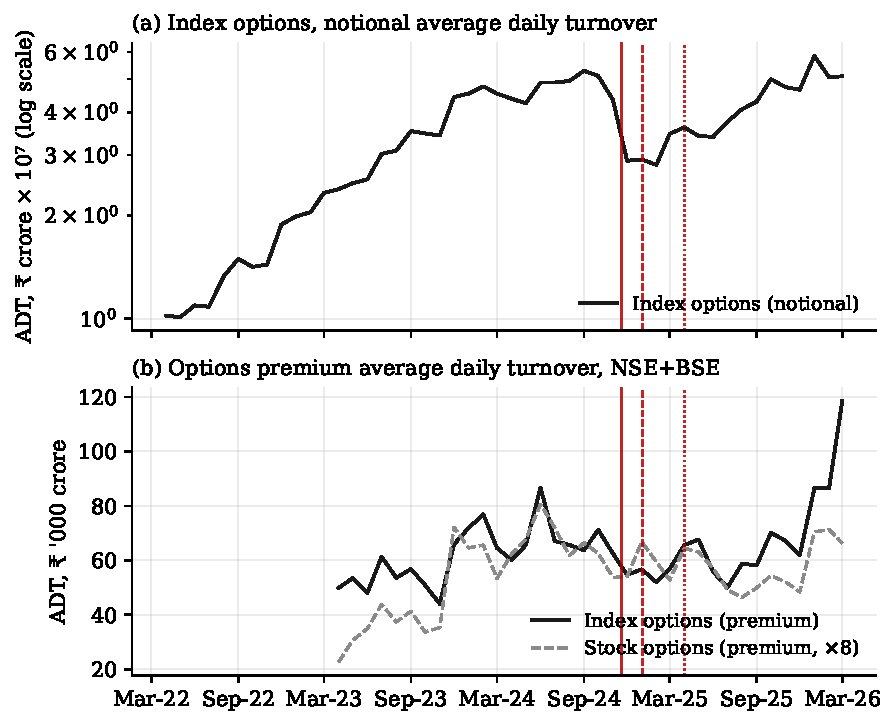
\includegraphics[width=0.86\textwidth]{fig1_series.pdf}
\caption{Index-options turnover, market-wide (NSE+BSE), April 2022--March
2026. Vertical lines mark the three reform waves (20 November 2024;
January 2025; 1 April 2025). Panel (b) overlays stock-options premium ADT
(scaled $\times 8$ for visibility), the control series.}
\label{fig:series}
\end{figure}

\section{Empirical Strategy}\label{sec:method}

\subsection{Difference-in-differences with a within-market control}

The reform package applies to \emph{index} derivatives only. Single-stock
options are our primary control: they trade on the same platforms, face the
same taxes (including the October 2024 STT increase), clear through the same
intermediaries, and are exposed to the same market cycle, but none of the
six measures in Table~\ref{tab:measures} applies to them.\footnote{Stock
derivatives position limits and ban-period rules were modified only later
(May 2025 circular), in the direction of \emph{loosening}; this would bias
our estimates toward zero. Index \emph{futures}, by contrast, are not a
valid control: the contract-value band and intraday position monitoring
apply to index derivatives generally, futures included.} One
microstructural asymmetry deserves note:
since October 2019, single-stock derivatives settle by physical delivery,
with delivery margins that escalate over the final days before expiry,
whereas index options are cash-settled. Episodes of market stress can
therefore move stock-options turnover through a settlement-friction channel
that does not operate on index options. The direction of any induced bias
is ambiguous---forced early square-offs of in-the-money positions raise
measured turnover, while deterred expiry-week positioning lowers it---and
our conclusions do not rest on stock options alone: the short-run relative
contraction is visible against stock futures and the cash market as well
(Tables~\ref{tab:its} and~\ref{tab:robust}). The estimating equation on the
two-group monthly panel is
\begin{equation}
\ln Y_{gt} \;=\; \alpha_g + \lambda_t + \beta\, \big(\mathrm{Index}_g \times
\mathrm{Post}_t\big) + \varepsilon_{gt},
\label{eq:did}
\end{equation}
where $Y_{gt}$ is ADT of group $g \in \{\text{index options},
\text{stock options}\}$ in month $t$, $\alpha_g$ are group effects,
$\lambda_t$ month effects, and $\mathrm{Post}_t = \mathbf{1}\{t \geq
\text{Nov 2024}\}$. With two groups and one adoption date,
equation~\eqref{eq:did} is a canonical $2\times2$ design: the negative-weight
pathologies of staggered two-way fixed effects
\citep{goodmanbacon2021,callawaysantanna2021,sunabraham2021} do not arise.

Inference with two groups cannot rely on clustering. Following
\citet{donaldlang2007} and \citet{bertrand2004}, we collapse the panel to the
monthly log difference $\Delta_t \equiv \ln Y_{\text{idx},t} - \ln
Y_{\text{stk},t}$ and estimate
\begin{equation}
\Delta_t \;=\; \mu + \beta\, \mathrm{Post}_t + u_t,
\label{eq:collapsed}
\end{equation}
with Newey--West HAC standard errors (six lags) \citep{neweywest1987}. The
point estimate of $\beta$ is numerically identical to
equation~\eqref{eq:did}. Equation~\eqref{eq:collapsed} also makes the nature
of the design explicit: with one treated and one control series, this is in
effect an interrupted time series on a differenced outcome, and all
inference is time-series inference---identification comes from the timing
of the treatment, not from cross-sectional variation across many treated
units. We choose six lags to allow serial correlation of up to half a year,
a longer window than automatic bandwidth rules would select at $T=48$, as a
conservative default.

\subsection{Differential trends and the trend-adjusted estimator}

Parallel trends is the key threat: index options were on a steeper growth
path than stock options before the reforms. In the pre-period the gap
$\Delta_t$ trends upward at $2.20$ log points per month
($\hat{\gamma}=0.022$; HAC $p = 0.002$) for notional and downward at
$3.34$ log points per month ($-0.033$; $p<0.001$) for premium. A constant
$\beta$ in equation~\eqref{eq:collapsed} is therefore biased toward zero for
notional (the counterfactual gap would have kept widening) and away from
zero for premium. Our preferred specification allows a group-specific linear
trend and a post-treatment trend break:
\begin{equation}
\Delta_t \;=\; \mu + \gamma\, t + \beta\, \mathrm{Post}_t
+ \delta\,(t - t_0)\,\mathrm{Post}_t + u_t,
\label{eq:ta}
\end{equation}
where $t_0$ is the first treated month. Here $\beta$ is the on-impact level
shift relative to the extrapolated differential trend and $\beta +
h\,\delta$ the implied gap at horizon $h$. The estimand is thus the effect
of the reform package as implemented on index-options ADT relative to stock
options, net of a differential pre-trend approximated as linear. Linear
extrapolation of a boom
trend is a strong assumption at long horizons---exactly the concern
formalized by \citet{rambachanroth2023}---so we emphasize short horizons
($h \leq 6$), report the average post-window deviation from trend, and treat
long-horizon extrapolations as bounds rather than estimates. We also report
event-study versions (the path of $\Delta_t$ relative to October 2024,
detrended on pre-period coefficients only) and placebo estimates that assign
a false adoption date of November 2023 within the pre-period, in the spirit
of \citet{conleytaber2011}.

\subsection{Interrupted time series}

For each series separately we estimate a seasonal interrupted-time-series
(ITS) model,
\begin{equation}
\ln Y_t = \alpha + \beta_1 t + \beta_2 \mathrm{Post}_t
+ \beta_3 (t - t_0)\mathrm{Post}_t + \textstyle\sum_{m}\theta_m
\mathbf{1}\{\text{month}=m\} + \epsilon_t,
\label{eq:its}
\end{equation}
with Newey--West errors. We use the ITS estimates not as causal effects but
as a decomposition device: comparing the break in the treated series with
breaks in untargeted series (stock options, stock futures, cash) reveals how
much of the raw collapse is market-wide.

\subsection{Cohort difference-in-differences}

SEBI's July 2025 study (Table~8) reports unique traders in six total-turnover
buckets for three six-month windows: December--May of 2022--23, 2023--24,
and 2024--25. The tripling of minimum contract size binds hardest on
small-ticket traders, so we define cohorts with six-month turnover below
\(\text{\rupee}\)10 lakh as exposed and estimate, on log growth rates
$g_{cw} = \Delta \ln N_{cw}$ across the two window-to-window transitions,
\begin{equation}
g_{cw} = \phi\,\mathrm{Exposed}_c + \psi\, \mathrm{Post}_w
+ \theta\,\big(\mathrm{Exposed}_c \times \mathrm{Post}_w\big) + e_{cw}.
\label{eq:cohort}
\end{equation}
With six cohorts and two periods, asymptotic inference is unreliable; we
therefore compute exact permutation $p$-values over all $\binom{6}{3}=20$
possible exposure assignments \citep{conleytaber2011}.

\section{Aggregate Turnover Results}\label{sec:results}

\subsection{Main estimates}

Table~\ref{tab:main} presents the turnover results. Columns (1)--(2) report
the unadjusted DiD of equation~\eqref{eq:collapsed} over the full window
(through March 2026); columns (3)--(4) end the sample in March 2025,
isolating the immediate post-reform period and predating the May 2025
circular and the July 2025 enforcement action; columns (5)--(6) report the
trend-adjusted specification of equation~\eqref{eq:ta}.

\begin{table}[H]
\centering
\caption{Effect of the 2024--25 curbs on index-options turnover:
difference-in-differences vs.\ stock options}
\label{tab:main}
\small
\begin{threeparttable}
\begin{tabular}{lcccccc}
\toprule
 & \multicolumn{2}{c}{Unadjusted, full} &
 \multicolumn{2}{c}{Unadjusted, $\leq$ Mar-25} &
 \multicolumn{2}{c}{Trend-adjusted, full} \\
\cmidrule(lr){2-3}\cmidrule(lr){4-5}\cmidrule(lr){6-7}
 & (1) & (2) & (3) & (4) & (5) & (6) \\
 & Notional & Premium & Notional & Premium & Notional & Premium \\
\midrule
Index $\times$ Post ($\beta$) & 0.033 & $-$0.072 & $-$0.167 & $-$0.210 & $-$0.573 & $-$0.007 \\
 & (0.138) & (0.114) & (0.110) & (0.103) & (0.148) & (0.058) \\
 & [0.809] & [0.528] & [0.128] & [0.042] & [0.000] & [0.905] \\
Post $\times$ trend ($\delta$) & & & & & 0.009 & 0.059 \\
 & & & & & (0.008) & (0.010) \\
Pre-period diff.\ trend ($\gamma$) & & & & & 0.022 & $-$0.033 \\
 & & & & & (0.007) & (0.006) \\
\midrule
Implied gap at 6 months & & & & & $-$0.520 & \\
Mean gap, Nov-24--May-25 & & & & & $-$0.557 & 0.240 \\
\quad (percent) & & & & & $-$42.7\% & \\
Months & 48 & 36 & 36 & 24 & 48 & 36 \\
\bottomrule
\end{tabular}
\begin{tablenotes}\footnotesize
\item Notes: Dependent variable is $\Delta_t = \ln(\text{index-options
ADT}) - \ln(\text{stock-options ADT})$, market-wide (NSE+BSE).
Newey--West standard errors (6 lags) in parentheses; $p$-values in
brackets. ``Post'' $= \mathbf{1}\{t\geq \text{Nov 2024}\}$.
Columns (5)--(6) estimate equation~\eqref{eq:ta}; the implied gap at
horizon $h$ is $\beta + h\delta$. The premium column (6) is dominated by
the reversal of the premium-to-notional compression trend; see
Section~\ref{subsec:composition}. Percent effects are $100(e^{\beta}-1)$.
\end{tablenotes}
\end{threeparttable}
\end{table}

Three patterns stand out. First, the unadjusted full-window DiD is
approximately zero: over 17 post months, index-options turnover ends up
where the two-group comparison alone would predict. This is \emph{not}
evidence of no effect; it reflects offsetting forces---an immediate
contraction followed by recovery and adaptation---combined with a
counterfactual (column 1) that ignores index options' steeper pre-trend.
Second, restricting to the immediate post window, index options
underperformed stock options by 15--19\% (columns 3--4; premium significant
at 5\%). Third, the preferred trend-adjusted estimates (column 5) show a
large and precisely estimated on-impact collapse in relative notional
turnover: 57 log points ($\hat{\beta}=-0.573$; $-44\%$; $p<0.001$), a
six-month gap of 52 log points, and an average November-to-May shortfall
of 56 log points ($-0.557$),
i.e.\ notional activity ran at about 57\% of its counterfactual level. The
positive but insignificant $\delta$ indicates slow relative recovery of
roughly 0.9 log points per month. In column (6) the object of interest is
the trend break $\delta$, not the level shift: the premium result \emph{is}
the reversal of the compression trend
(Section~\ref{subsec:composition}).

The conclusions do not hinge on stock options as the sole comparator. The
ITS decomposition below shows the same asymmetric break against stock
futures and the cash market, and Table~\ref{tab:robust} shows that the
full-window DiD with stock futures as the control ($0.161$, s.e.\ $0.168$)
matches the stock-options result almost exactly: the identification rests
on triangulation across three untargeted segments, not on a single control
series.

Figure~\ref{fig:didgap} displays the identifying variation transparently:
the log gap between index- and stock-options notional ADT, its pre-period
linear trend, and the post-reform shortfall. The gap drops discretely in
November--December 2024, bottoms after the January 2025 contract-size
increase, and then narrows gradually without returning to trend by March
2026. Figure~\ref{fig:es} shows the event-study version: pre-period
detrended coefficients fluctuate around zero with no anticipation in the
announcement window (October 2024), followed by a sharp break at
implementation.

\begin{figure}[H]
\centering
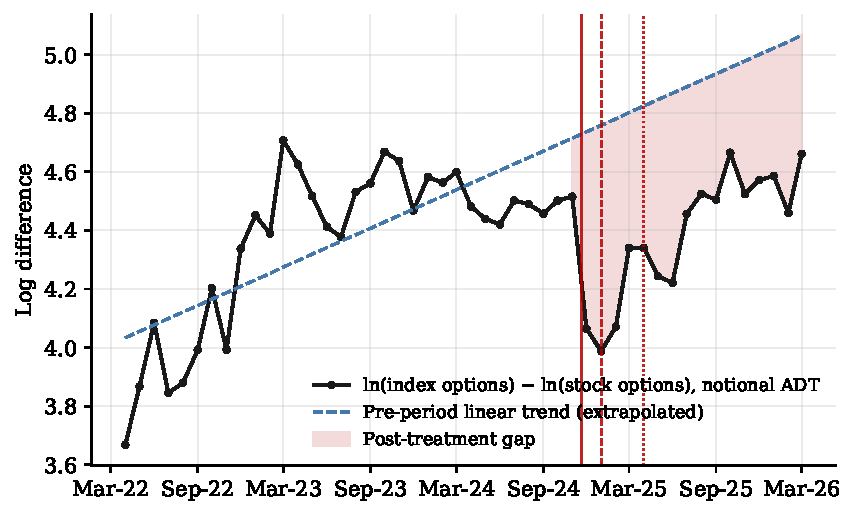
\includegraphics[width=0.88\textwidth]{fig2_did_gap.pdf}
\caption{The identifying gap. Solid line: $\ln(\text{index-options
notional ADT}) - \ln(\text{stock-options notional ADT})$, market-wide.
Dashed line: linear trend fitted on the pre-period (April 2022--October
2024) and extrapolated. Shaded area: post-treatment shortfall. Vertical
lines: reform waves.}
\label{fig:didgap}
\end{figure}

\begin{figure}[H]
\centering
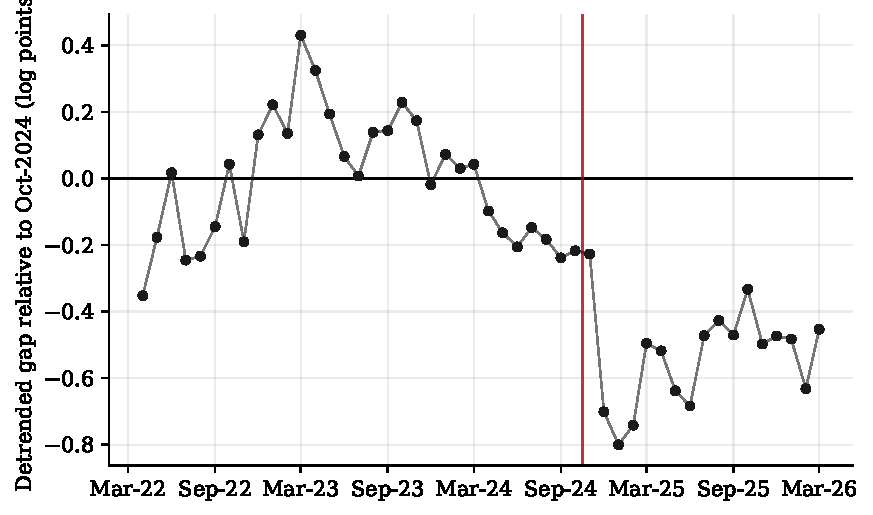
\includegraphics[width=0.88\textwidth]{fig3_event_study.pdf}
\caption{Event-study representation: monthly gap relative to October 2024,
detrended using pre-period observations only. The vertical line marks the
first reform wave (20 November 2024).}
\label{fig:es}
\end{figure}

\subsection{Decomposition: how much of the raw decline was the reform?}

The raw year-on-year decline in market-wide index-options notional ADT for
December--May windows is $-29.2\%$---SEBI's headline number. The ITS
estimates in Table~\ref{tab:its} put the naive level break for index-options
notional at $-0.838$ log points ($-57\%$), but the same specification
applied to untargeted segments yields breaks of $-0.260$ (stock options),
$-0.269$ (stock futures), and $-0.337$ (cash): a market-wide contraction of
roughly 23--29\% coincided with the reforms. Netting this out---which is
what the DiD does---attributes roughly 43\% (trend-adjusted, short-run) of
the treated-series collapse to the reforms and the remainder to the common
cycle. The lesson for policy evaluation is direct: before--after comparisons
around November 2024 overstate the causal effect of the curbs by roughly a
third.

\begin{table}[H]
\centering
\caption{Interrupted time series, by segment (log ADT, monthly)}
\label{tab:its}
\small
\begin{threeparttable}
\begin{tabular}{lccccc}
\toprule
 & (1) & (2) & (3) & (4) & (5) \\
 & Index opt. & Index opt. & Stock opt. & Stock fut. & Cash \\
 & (notional) & (premium) & (notional) & & \\
\midrule
Level break ($\beta_2$) & $-$0.838 & $-$0.429 & $-$0.260 & $-$0.269 & $-$0.337 \\
 & (0.091) & (0.064) & (0.056) & (0.090) & (0.077) \\
 & [0.000] & [0.000] & [0.000] & [0.003] & [0.000] \\
Slope change ($\beta_3$) & $-$0.023 & 0.008 & $-$0.031 & $-$0.029 & $-$0.025 \\
 & (0.005) & (0.006) & (0.005) & (0.007) & (0.006) \\
Pre-trend ($\beta_1$) & 0.060 & 0.022 & 0.038 & 0.033 & 0.037 \\
$R^2$ & 0.952 & 0.618 & 0.900 & 0.815 & 0.821 \\
Months & 48 & 36 & 48 & 48 & 48 \\
\bottomrule
\end{tabular}
\begin{tablenotes}\footnotesize
\item Notes: equation~\eqref{eq:its} with calendar-month dummies;
Newey--West standard errors (6 lags) in parentheses, $p$-values in
brackets. The comparison of column (1) with columns (3)--(5) shows that
untargeted segments also broke downward at the reform date, reflecting
the concurrent market correction; ITS breaks are therefore upper bounds
on the causal effect.
\end{tablenotes}
\end{threeparttable}
\end{table}

\subsection{Composition: notional versus premium}\label{subsec:composition}

The reforms compressed notional turnover far more than premium turnover:
$-29.2\%$ versus $-13.0\%$ year on year. Mechanically, eliminating four of
five weekly expiries removes the cheapest, shortest-dated contracts---those
with the lowest premium-to-notional ratios---and tripling the lot size
truncates the smallest trades. The trend-adjusted premium regression
(Table~\ref{tab:main}, column 6) makes the compositional shift precise: the
pre-period premium gap was \emph{falling} at 3.3 log points per month
(options were becoming progressively cheaper relative to their notional as
the weekly-expiry share grew), and after the reforms this trend reversed to
$+5.9$ log points per month ($p<0.001$). The average price of traded option
exposure rose. In economic terms, the reforms did not proportionally reduce
the rupee amount spent on option purchases; they eliminated the
highest-leverage, lottery-like end of the product spectrum---precisely the
segment SEBI's studies associate with the most concentrated retail losses.

Two caveats bound this interpretation. First, premium turnover is an
imperfect welfare metric: it measures buyers' outlay, not net economic
exposure, and is silent on the risk borne by option writers. Second, part
of the ratio's rise could in principle reflect the elevated implied
volatility of the October 2024--February 2025 correction, which
mechanically raises premia per unit of notional; that the reversal persists
well after the correction ended---the post-reform ratio trend runs through
March 2026---points to composition rather than transient option repricing,
but without contract-level moneyness data we cannot decompose the two
channels formally. The compositional pattern also contrasts instructively
with the 2015 lot-size episode, in which constrained retail flow
\emph{escaped} into cheaper, deeper out-of-the-money contracts
\citep{agarwal2025animal}: by removing four of five weekly expiries at the
same time as it raised the minimum ticket, the 2024--25 package closed the
avenue-shifting margin that undid the earlier, single-instrument
intervention.

\section{Participation and Heterogeneity}\label{sec:hetero}

\subsection{Who exited}

Unique individual traders in equity derivatives fell from 84.1 lakh
(December 2023--May 2024) to 67.6 lakh (December 2024--May 2025), $-20\%$,
after rising 54\% the previous year. Figure~\ref{fig:cohorts} shows the
cohort pattern that provides the paper's central mechanism evidence for
the contract-size channel: growth reversals are
monotonically decreasing in trader size. The smallest bucket
($<\text{\rupee}$10,000 of six-month turnover) swung from $+81$ log points
of growth pre-reform to $-36$ post; the \(\text{\rupee}\)1--10 crore bucket
swung from $+28$ to $-4$.

\begin{figure}[H]
\centering
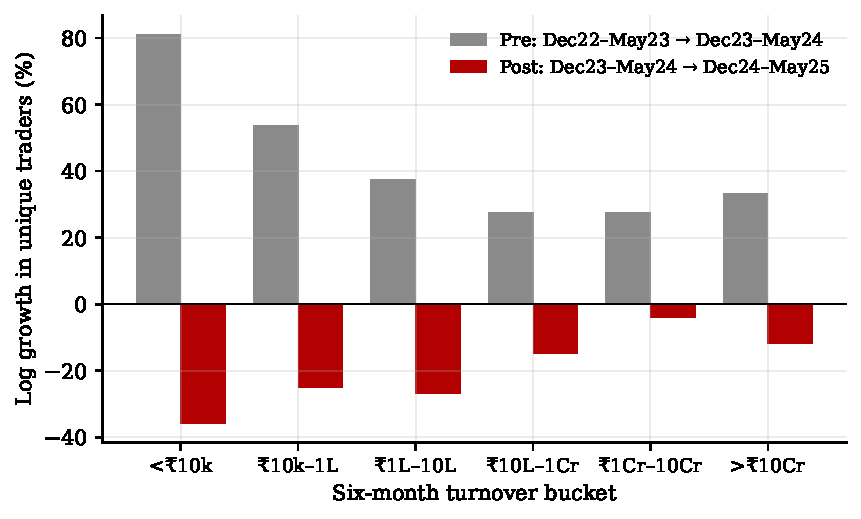
\includegraphics[width=0.85\textwidth]{fig4_cohorts.pdf}
\caption{Log growth in unique traders by six-month turnover bucket,
pre-reform transition (December 2022--May 2023 $\rightarrow$ December
2023--May 2024) versus post-reform transition (December 2023--May 2024
$\rightarrow$ December 2024--May 2025). Source: authors' calculations from
\citet{sebi2025comparative}, Table~8.}
\label{fig:cohorts}
\end{figure}

Estimating equation~\eqref{eq:cohort} with the three sub-\(\text{\rupee}\)10-lakh
buckets as exposed yields $\hat{\theta} = -0.468$ (HC1 s.e.\ 0.137,
$p=0.001$): small-ticket cohorts lost an additional 47 log points of
participation growth relative to large-ticket cohorts, over and above the
common post-reform reversal. Exact permutation inference over all 20
exposure assignments gives $p = 0.10$---the realized assignment produces the
second-largest $|\hat{\theta}|$ of the 20, where 0.05 is the smallest
attainable value with six cohorts. Given the monotone dose--response
visible in Figure~\ref{fig:cohorts} (the effect declines steadily across all
six buckets rather than depending on one outlier), we read the cohort
evidence as consistent with the contract-size channel: tripling the
minimum ticket priced the smallest traders out first. Two further
design-based checks reinforce this reading. Treating exposure continuously
rather than as a binary---regressing cohort growth on the log midpoint of
the turnover bucket, a post indicator, and their interaction---yields a
dose--response slope of $0.065$ log points of participation growth per log
rupee of cohort size after the reform (HC1 s.e.\ $0.016$), and the Spearman
rank correlation between cohort size and the pre-to-post growth swing is
$0.83$ ($p=0.042$, $n=6$): larger cohorts were systematically more
insulated.

The exit was derivatives-specific, not a retreat from equity markets.
Total demat accounts across NSDL and CDSL rose from 15.1 crore at
end-March 2024 to 19.2 crore at end-March 2025---growth of 27\% during the
very year in which unique derivatives traders fell 20\%---and reached
22.5 crore by early 2026.\footnote{NSDL: 358 lakh (Mar-2024)
$\rightarrow$ 395 lakh (Mar-2025) $\rightarrow$ 444 lakh; CDSL: 1,156
$\rightarrow$ 1,530 $\rightarrow$ 1,801 lakh. Source: SEBI Monthly
Bulletin depository-statistics tables (April 2025 and April 2026 issues).}
New investors kept entering the securities market throughout the reform
window; what contracted was participation in the targeted product class.

Two features of the cohort data deserve emphasis. First, average traded
value \emph{within} buckets barely moved (SEBI Table~9 reports within-bucket
changes of 0--8\%), so the participation declines are an extensive-margin
phenomenon---traders exiting---rather than incumbents shrinking within
buckets. Second, the pre-period cohort growth rates reveal the boom's
recruitment pattern: the smallest cohort was growing fastest before the
reforms (+81 log points), meaning the policy interrupted an inflow of
precisely the marginal, small, inexperienced traders whose loss rates SEBI's
studies show to be the worst.

\subsection{Quarterly dynamics of participation and losses}

Figure~\ref{fig:quarterly} tracks FY2025 by quarter. Unique traders declined
from 61.4 lakh in Q1 to 42.7 lakh in Q4 ($-30\%$), with the largest
single-quarter drop in Q4---the first full quarter with all major measures
in force. Aggregate net losses peaked at \(\text{\rupee}\)33,661 crore in
Q3 and fell 26\% in Q4 (\(\text{\rupee}\)24,745 crore); average per-person
losses fell 8\%. The per-trader improvement is modest: the loss-maker share
remained at 86.4\% in Q4, against 84.5\% in Q1. On the earliest available
evidence, the curbs shrank the base of exposed traders substantially but
improved the odds of the remaining traders only marginally.

\begin{figure}[H]
\centering
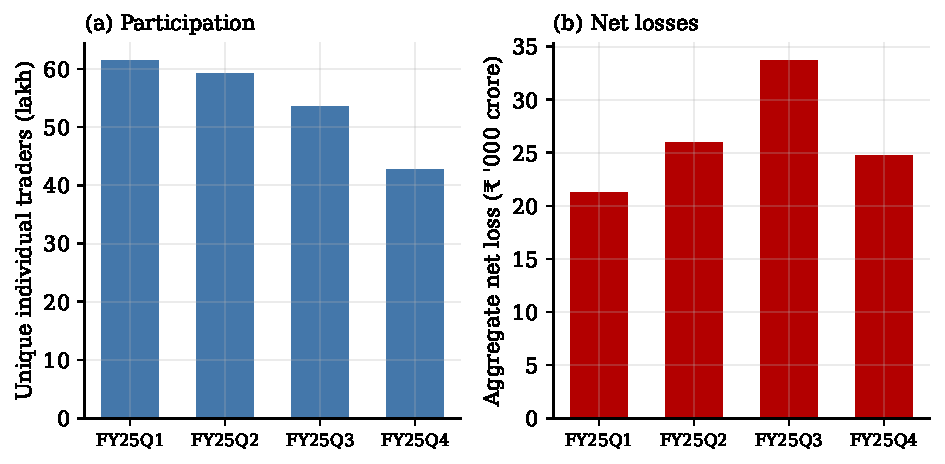
\includegraphics[width=0.9\textwidth]{fig5_quarterly.pdf}
\caption{Quarterly participation and aggregate net losses of individual
traders in equity derivatives, FY2025. Source:
\citet{sebi2025comparative}, Table~12 (sample of top-13 brokers,
$\approx$96 lakh unique traders).}
\label{fig:quarterly}
\end{figure}

\section{Substitution and Falsification}\label{sec:subst}

\subsection{No migration to the cash market}

A stated concern around the reforms was that displaced speculation would
migrate to the cash segment (particularly intraday equity trading). The data
show the opposite: cash-market ADT fell 9.6\% year on year over the
December--May comparison window, and its ITS level break ($-0.337$) is
statistically indistinguishable from the breaks in stock options and stock
futures (Table~\ref{tab:its}). Figure~\ref{fig:subst} plots all series
indexed to their May--October 2024 average: no untargeted segment rises as
index options fall. The adjustment margin was exit---consistent with the
20\% decline in unique traders---rather than substitution across the
products we observe. This conclusion is bounded by the panel's coverage:
it speaks to aggregate exchange turnover in equity segments. Substitution
into channels outside the panel---commodity or currency derivatives,
offshore venues, or a shift from intraday to delivery-based activity within
the cash aggregate---cannot be ruled out; what the data establish is that
the cash market in aggregate absorbed no measurable inflow.

\begin{figure}[H]
\centering
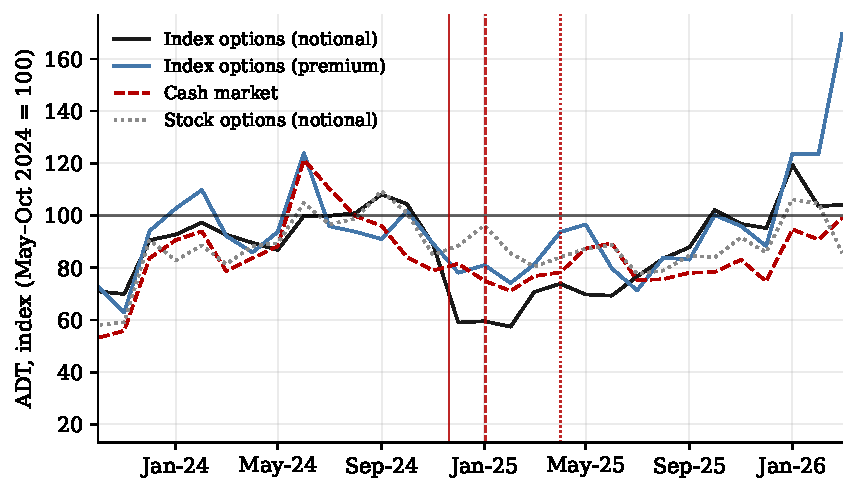
\includegraphics[width=0.88\textwidth]{fig6_substitution.pdf}
\caption{Average daily turnover by segment, indexed to the May--October
2024 mean ($=100$). If curbed index-options activity had migrated to other
segments, their indices would rise after November 2024; none does.}
\label{fig:subst}
\end{figure}

\subsection{Exchange substitution}

Cross-exchange migration, by contrast, was substantial. Re-estimating the
full-window notional DiD on NSE-only data yields $\beta = -0.374$
($p<0.001$; $-31\%$), against $\approx 0$ market-wide. The wedge reflects
BSE's rising share: with NSE's weekly products consolidated to Nifty alone,
activity continued shifting toward BSE's surviving weekly Sensex contract
through FY2026. Studies that measure the reforms' effects on NSE data
alone will therefore overstate the aggregate decline by conflating policy
impact with venue substitution---a general lesson for evaluating exchange
regulation in fragmented markets. Figure~\ref{fig:bseshare} traces the
migration directly: BSE's share of market-wide index-options ADT rose from
23.5\% (notional) and 12.7\% (premium) in October 2024 to 44.1\% and
27.9\% by March 2026, with no reversal after any reform wave.

\begin{figure}[H]
\centering
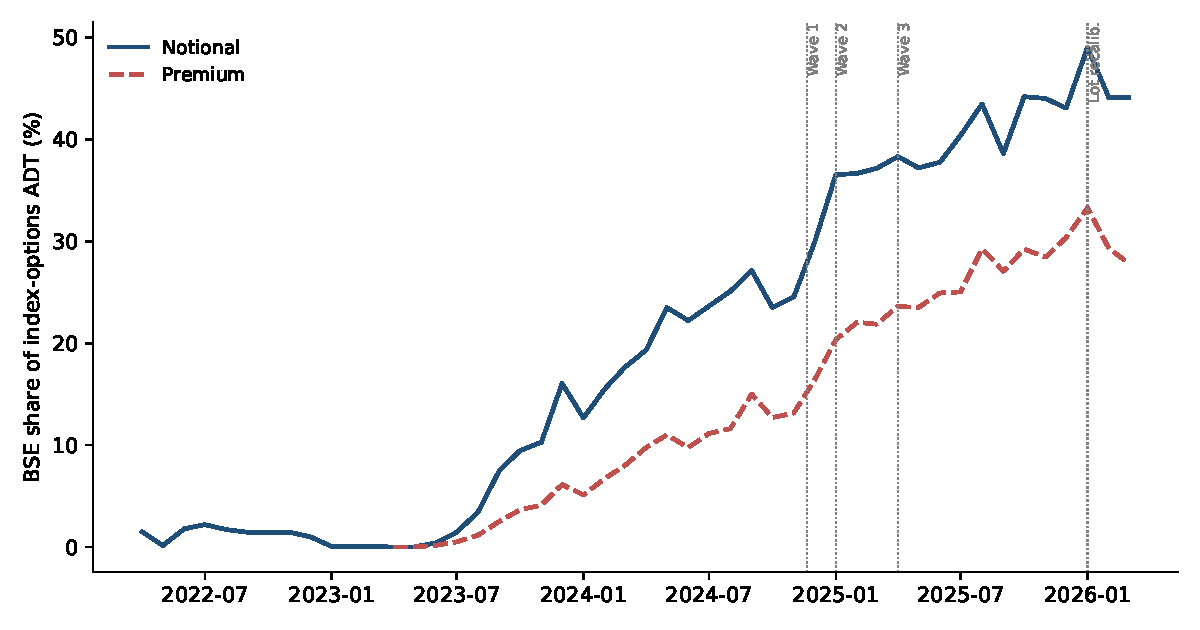
\includegraphics[width=0.85\textwidth]{fig8_bse_share.pdf}
\caption{BSE's share of market-wide index-options average daily turnover,
April 2022--March 2026. Dotted vertical lines mark the three reform waves
and the January 2026 lot-size recalibration. Source: authors' calculations
from SEBI Monthly Bulletin annexure tables (NSE and BSE panels).}
\label{fig:bseshare}
\end{figure}

\section{Robustness}\label{sec:robust}

Table~\ref{tab:robust} collects robustness checks on the collapsed-series
DiD.

\begin{table}[H]
\centering
\caption{Robustness of the difference-in-differences estimates}
\label{tab:robust}
\small
\begin{threeparttable}
\begin{tabular}{lccc}
\toprule
Specification & $\beta$ & s.e. & $N$ (months) \\
\midrule
\multicolumn{4}{l}{\emph{Panel A: placebo adoption date (Nov 2023), pre-period only}}\\
\quad Notional & 0.243 & (0.140) & 31 \\
\quad Premium & $-$0.387 & (0.065) & 19 \\
\addlinespace
\multicolumn{4}{l}{\emph{Panel B: sample perturbations (full window, unadjusted)}}\\
\quad Drop transition months (Nov--Dec 2024), notional & 0.048 & (0.141) & 46 \\
\quad Drop transition months (Nov--Dec 2024), premium & $-$0.066 & (0.113) & 34 \\
\quad Drop Jul--Aug 2025 (enforcement action), notional & 0.021 & (0.141) & 46 \\
\quad Drop Jul--Aug 2025 (enforcement action), premium & $-$0.072 & (0.117) & 34 \\
\addlinespace
\multicolumn{4}{l}{\emph{Panel C: alternative control and venue}}\\
\quad Control = stock futures, notional & 0.161 & (0.168) & 48 \\
\quad NSE only, notional & $-$0.374 & (0.106) & 48 \\
\bottomrule
\end{tabular}
\begin{tablenotes}\footnotesize
\item Notes: all rows estimate equation~\eqref{eq:collapsed}
(equation~\eqref{eq:ta} logic applies as in the main table) with
Newey--West (6-lag) standard errors. Panel A assigns a false adoption date
of November 2023 and estimates on pre-period data only. The significant
premium placebo reflects the strong pre-existing premium-compression
trend and motivates the trend-adjusted specification, whose placebo
analogue is the pre-trend coefficient itself. Panel C's NSE-only estimate
bundles the policy effect with NSE$\rightarrow$BSE migration.
\end{tablenotes}
\end{threeparttable}
\end{table}

Three points. First, the notional placebo is small, positive, and
insignificant at 5\% ($0.243$, $p=0.083$); the premium placebo is large and
significant, but this is exactly the manifestation of the premium series'
strong secular trend that our trend-adjusted estimator is built to absorb---
after trend adjustment the ``placebo'' object is the pre-trend itself, which
is estimated, not assumed. Second, results are insensitive to dropping the
implementation-transition months and the enforcement-action months. Third,
using stock futures as an alternative control yields the same qualitative
conclusion (near-zero full-window unadjusted DiD); no alternative control
overturns the short-run contraction, which is visible against every
untargeted segment.

Beyond Table~\ref{tab:robust}, the cohort result survives its own design-based
test (permutation inference, Section~\ref{sec:hetero}), and the
aggregate-turnover conclusions do not rest on any single data vintage: the
panel reproduces SEBI's independently published window aggregates to within
0.2--4\% (Section~\ref{sec:data}).

Two further checks address inference and the post period's non-uniform
treatment intensity. First, the trend-adjusted notional estimate is
insensitive to the HAC bandwidth: across Newey--West lags of 2 to 12 the
point estimate is unchanged ($-0.573$) and its standard error ranges only
from $0.131$ to $0.148$, with $p<10^{-3}$ throughout. Second, splitting the
post indicator at the January 2026 lot-size recalibration---the design
remains a two-group, single-adoption comparison; the post period is merely
partitioned---locates the recovery in time: in the unadjusted collapsed
series, the index--stock gap averages $-0.004$ (s.e.\ $0.138$) over
November 2024--December 2025 but $+0.206$ (s.e.\ $0.105$) over
January--March 2026, the three months after the exchanges lowered the
Nifty lot from 75 to 65. With only three post-recalibration months we read
this as descriptive, but it is consistent with
Section~\ref{sec:background}'s interpretation that part of the late-sample
turnover recovery is rule-driven rather than purely behavioral.

Finally, the on-impact break does not depend on the linearity of the
differential pre-trend. Allowing a quadratic pre-trend yields a level shift
of $-0.396$ (s.e.\ $0.077$); a piecewise-linear pre-period (kink at the
pre-sample midpoint) yields $-0.331$ (s.e.\ $0.071$); both remain
significant at $p<10^{-4}$. What curvature does affect is
\emph{extrapolated magnitudes}: a concave quadratic extrapolated over the
post window implies the boom would have reversed on its own, an unstable
counterfactual at multi-month horizons. This is precisely why magnitude
statements in this paper are anchored to the linear-trend and no-trend
bracket of Section~\ref{subsec:sens} rather than to any higher-order
extrapolation, and why the discrete break---robust across all three trend
specifications---is the primary causal object.

\subsection{Sensitivity to the counterfactual trend}\label{subsec:sens}

The trend-adjusted estimate extrapolates the estimated pre-period
differential trend ($\hat{\gamma} = 0.022$ log points per month). Following
the logic of \citet{rambachanroth2023}, Figure~\ref{fig:sens} recomputes the
average November 2024--May 2025 effect under \emph{every} assumed
counterfactual trend $\gamma$ in a wide grid, anchored at the October 2024
fitted level. The estimate is $-0.557$ at $\hat{\gamma}$ and remains
$-0.469$ ($-37\%$) with no trend adjustment at all ($\gamma = 0$). The
breakdown value at which the effect reaches zero is $\gamma^{*} = -0.117$:
the index--stock options gap would have had to be \emph{shrinking} at
11.7 log points per month absent the reforms---a trend opposite in sign to
the estimated one, 19.7 standard errors below it, and more than five times
its magnitude. No plausible violation of the trend assumption overturns the
short-run contraction; the honest bracket for the short-run effect is
$[-43\%, -37\%]$, spanned by the with- and without-trend estimates.

\begin{figure}[H]
\centering
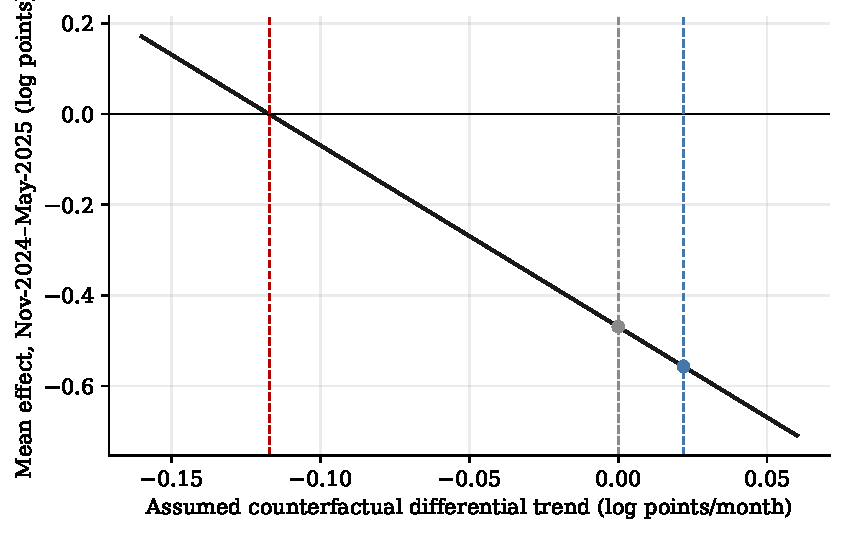
\includegraphics[width=0.8\textwidth]{fig7_sensitivity.pdf}
\caption{Sensitivity of the short-run effect to the assumed counterfactual
differential trend, in the spirit of \citet{rambachanroth2023}. The mean
November 2024--May 2025 effect is plotted against the counterfactual trend
$\gamma$ imposed on the index--stock options log gap (anchored at the
October 2024 fitted level). Reference lines mark no adjustment
($\gamma=0$), the estimated pre-trend $\hat{\gamma}=0.022$
(s.e.\ $0.007$), and the breakdown value $\gamma^{*}=-0.117$.}
\label{fig:sens}
\end{figure}

\section{Discussion}\label{sec:discussion}

\subsection{Interpreting the pattern of effects}

Taken together, the estimates describe a regulation that worked through
exactly the channels its design implies, with a mix of intended and
unintended consequences:

\emph{Scale.} The short-run contraction in targeted activity was large
(roughly $-43\%$ against counterfactual in notional terms) and front-loaded
around the weekly-expiry rationalization and the contract-size increase---
the two measures that mechanically destroy trade opportunities rather than
merely repricing them.

\emph{Composition.} The premium-to-notional ratio reversed a multi-year
compression trend, implying the surviving flow is concentrated in larger,
more expensive, less lottery-like contracts. If the policy objective is
framed as reducing the availability of cheap, high-leverage, near-expiry
speculation to small retail traders, the composition evidence indicates
success on that specific margin.

\emph{Incidence.} Participation declines were concentrated among the
smallest traders---mechanically so, since a \(\text{\rupee}\)15--20 lakh
minimum ticket binds only on them. Whether this is welfare-improving
depends on one's model of the marginal small trader. Under the
behavioral-losses view supported by SEBI's profitability studies (91\% of
individuals losing, average loss exceeding \(\text{\rupee}\)1 lakh per
person), removing small traders from a negative-expected-value game is
protective. Under a consumer-sovereignty view, the same fact pattern is a
paternalistic exclusion of small players from a market that remains open to
the wealthy. The Q4-FY2025 data---losses per remaining trader down only
8\%, loss-maker share broadly unchanged---suggest the reform's protective
effect operates almost entirely through the extensive margin (fewer people
exposed) rather than by improving anyone's trading outcomes. This pattern
speaks to a live domestic policy debate: \citet{aggarwalmitra2026} argue
that poorly targeted derivatives interventions impose market-wide costs
without improving the outcomes of the traders they aim to protect. Our
evidence is consistent with the outcome half of that critique---per-trader
loss rates barely moved---while showing that the package did achieve a
large, targeted, and so-far durable reduction in the number of small
traders exposed.

\emph{Adaptation.} The aggregate turnover effect decayed within a year:
market-wide premium ADT exceeded pre-reform levels by Q4 FY2026. Mechanisms
visible in our data include venue substitution toward BSE's surviving weekly
product and re-concentration of activity in the permitted contracts;
mechanisms documented elsewhere include longer-dated positioning. In
addition, the January 2026 lot-size recalibration (Nifty 75 to 65)
mechanically lowered the minimum ticket by about 13\%, so part of the
late-sample recovery reflects a rule-driven relaxation of treatment
intensity rather than behavioral adaptation alone. The
participation decline, by contrast, shows no reversal through the latest
available cohort data. A regulation aiming at \emph{who} trades appears more
durable than one aiming at \emph{how much} is traded.

\subsection{Implications for market participants}

For brokers and exchanges, the results imply that the revenue shock from
derivatives curbs is better forecast from participation (client-count)
elasticities than from headline turnover, which recovers: discount brokers
whose economics depend on small-ticket order flow bear the persistent
incidence, while exchange premium-based fee pools recovered within five
quarters. For institutional traders and market makers, the compositional
shift toward higher premium-per-notional contracts and a single weekly
expiry per exchange concentrates gamma and expiry-day risk in fewer, larger
maturities---consistent with the regulator's follow-on May 2025 move to
delta-based (``future-equivalent'') open-interest metrics and expiry-day
standardization. For policymakers elsewhere confronting retail options
booms, the obvious parallel is the United States, where zero-days-to-expiry
(0DTE) contracts---daily-expiring S\&P~500 options that now account for
roughly half of SPX options volume---are dominated by small retail trades
with negative average returns \citep{beckmeyer2023zdte}. India ran the
restrictive counterfactual to the permissive US regime: the experiment
suggests contract-design levers (expiry frequency, minimum ticket size) can
achieve targeted de-risking quickly and regressively, but that
turnover-based success metrics will flatter the intervention only briefly.

\subsection{Limitations}

Our causal claims rest on aggregate, segment-level data; trader-level
microdata remain proprietary to SEBI and the exchanges. Three specific
limitations follow. First, with one treated and one control series,
inference relies on time-series variation (HAC), placebo dates, and design
transparency rather than cross-sectional clustering; we cannot rule out an
index-options-specific shock coincident with November 2024 other than the
reforms, though we know of no candidate---the market correction, STT change,
and enforcement shocks are all either common to the control or explicitly
tested. Second, the trend-adjusted counterfactual extrapolates a boom-era
differential trend; Section~\ref{subsec:sens} shows the short-run
conclusion survives every counterfactual trend short of an implausible
sign reversal 19.7 standard errors below the estimate, and the
unadjusted and trend-adjusted estimates bracket the effect at
$[-37\%, -43\%]$. Third, the cohort design has six units and two
periods; its permutation $p$-value (0.10) is bounded below by 0.05, and we
lean on the monotone dose--response pattern rather than the significance
threshold. Fourth, the control is not microstructurally identical to the
treated series: stock options settle physically, with escalating
expiry-week delivery margins, while index options settle in cash
(Section~\ref{sec:method} discusses the direction of any induced bias and
the untargeted-segment checks that bound it). Fifth, our substitution
analysis observes exchange-traded equity segments only; migration to
commodity, currency, or offshore products is outside the panel. Finally,
FY2023 premium data do not exist in the bulletin format, so premium
estimates use 19 pre-treatment months against 31 for notional, and the
premium results are correspondingly less well identified.

\section{Conclusion}\label{sec:conclusion}

SEBI's 2024--25 index-derivatives reforms are the sharpest regulatory
experiment yet run on a retail options boom. Exploiting the package's
exclusive targeting of index products, we estimate that the curbs reduced
index-options notional turnover by 37--43\% relative to counterfactual
in the six months after implementation, reversed a multi-year slide in the
premium-to-notional ratio, and pushed roughly one in five individual
traders---disproportionately the smallest---out of the equity derivatives
segment, with no detectable migration into the cash market at the
aggregate level. Aggregate turnover adapted and recovered within five
quarters---partly through migration to BSE's surviving weekly product and
partly through the exchanges' rule-driven January 2026 lot-size
recalibration; the contraction in participation did not reverse. The reforms, in short, succeeded quickly at their
compositional and participation objectives while their headline turnover
effect proved transitory---an instructive combination for regulators
weighing product-design interventions against transaction taxes, and a
caution against evaluating either by turnover alone.

Three extensions merit future work as data accumulate: trader-level
profitability after the reforms (does the surviving population's loss rate
fall?), the May 2025 delta-based open-interest framework as a second
experiment, and the cross-market comparison with the United States'
zero-days-to-expiry growth under a permissive regime.

\newpage
\begin{thebibliography}{99}

\bibitem[Agarwal et al.(2025)]{agarwal2025animal}
Agarwal, V., P. Ghosh, N.~R. Prabhala, and H. Zhao (2025).
Animal spirits on steroids: Evidence from retail options trading in India.
Working paper (SSRN 5430635).

\bibitem[Aggarwal and Mitra(2026)]{aggarwalmitra2026}
Aggarwal, N. and B. Mitra (2026).
Retail losses in India's derivatives market: A re-examination of the
evidence.
\emph{Ideas for India}, 29 April 2026.

\bibitem[Barber et al.(2009)]{barberleeliuodean2009}
Barber, B.~M., Y.-T. Lee, Y.-J. Liu, and T. Odean (2009).
Just how much do individual investors lose by trading?
\emph{Review of Financial Studies} 22(2), 609--632.

\bibitem[Bauer et al.(2009)]{bauer2009option}
Bauer, R., M. Cosemans, and P. Eichholtz (2009).
Option trading and individual investor performance.
\emph{Journal of Banking \& Finance} 33(4), 731--746.

\bibitem[Beckmeyer et al.(2023)]{beckmeyer2023zdte}
Beckmeyer, H., N. Branger, and L. Gayda (2023).
Retail traders love 0DTE options... but should they?
Working paper, University of M\"unster (SSRN 4404704).

\bibitem[Bertrand et al.(2004)]{bertrand2004}
Bertrand, M., E. Duflo, and S. Mullainathan (2004).
How much should we trust differences-in-differences estimates?
\emph{Quarterly Journal of Economics} 119(1), 249--275.

\bibitem[Boyer and Vorkink(2014)]{boyer2014expected}
Boyer, B.~H. and K. Vorkink (2014).
Stock options as lotteries.
\emph{Journal of Finance} 69(4), 1485--1527.

\bibitem[Bryzgalova et al.(2023)]{bryzgalova2023retail}
Bryzgalova, S., A. Pavlova, and T. Sikorskaya (2023).
Retail trading in options and the rise of the big three wholesalers.
\emph{Journal of Finance} 78(6), 3465--3514.

\bibitem[Callaway and Sant'Anna(2021)]{callawaysantanna2021}
Callaway, B. and P.~H.~C. Sant'Anna (2021).
Difference-in-differences with multiple time periods.
\emph{Journal of Econometrics} 225(2), 200--230.

\bibitem[Conley and Taber(2011)]{conleytaber2011}
Conley, T.~G. and C.~R. Taber (2011).
Inference with ``difference in differences'' with a small number of policy
changes.
\emph{Review of Economics and Statistics} 93(1), 113--125.

\bibitem[de Silva et al.(2024)]{dejong2024retail}
de Silva, T., K. Smith, and E.~C. So (2024).
Losing is optional: Retail option trading and expected announcement
volatility.
Working paper, MIT Sloan.

\bibitem[Donald and Lang(2007)]{donaldlang2007}
Donald, S.~G. and K. Lang (2007).
Inference with difference-in-differences and other panel data.
\emph{Review of Economics and Statistics} 89(2), 221--233.

\bibitem[Goodman-Bacon(2021)]{goodmanbacon2021}
Goodman-Bacon, A. (2021).
Difference-in-differences with variation in treatment timing.
\emph{Journal of Econometrics} 225(2), 254--277.

\bibitem[Heimer and Simsek(2019)]{heimersimsek2019}
Heimer, R. and A. Simsek (2019).
Should retail investors' leverage be limited?
\emph{Journal of Financial Economics} 132(3), 1--21.

\bibitem[Jones and Seguin(1997)]{jonesseguin1997}
Jones, C.~M. and P.~J. Seguin (1997).
Transaction costs and price volatility: Evidence from commission
deregulation.
\emph{American Economic Review} 87(4), 728--737.

\bibitem[Kumar(2009)]{kumar2009gambling}
Kumar, A. (2009).
Who gambles in the stock market?
\emph{Journal of Finance} 64(4), 1889--1933.

\bibitem[Lee et al.(2026)]{leeryuwebb2026}
Lee, J., D. Ryu, and R.~I. Webb (2026).
How do option contract sizes affect investor composition and market
quality?
\emph{Review of Derivatives Research} 29(1).

\bibitem[Newey and West(1987)]{neweywest1987}
Newey, W.~K. and K.~D. West (1987).
A simple, positive semi-definite, heteroskedasticity and autocorrelation
consistent covariance matrix.
\emph{Econometrica} 55(3), 703--708.

\bibitem[Rambachan and Roth(2023)]{rambachanroth2023}
Rambachan, A. and J. Roth (2023).
A more credible approach to parallel trends.
\emph{Review of Economic Studies} 90(5), 2555--2591.

\bibitem[SEBI(2023)]{sebi2023study}
Securities and Exchange Board of India (2023).
Analysis of profit and loss of individual traders dealing in equity
futures and options segment.
Study, Department of Economic and Policy Analysis, 25 January 2023.

\bibitem[SEBI(2024)]{sebi2024study}
Securities and Exchange Board of India (2024).
Analysis of profits and losses in the equity derivatives segment
(FY22--FY24).
Study, Department of Economic and Policy Analysis, 23 September 2024.

\bibitem[SEBI(2025)]{sebi2025comparative}
Securities and Exchange Board of India (2025).
Comparative study of growth in equity derivatives segment vis-\`a-vis cash
market after recent measures.
Research report, 7 July 2025.

\bibitem[Sun and Abraham(2021)]{sunabraham2021}
Sun, L. and S. Abraham (2021).
Estimating dynamic treatment effects in event studies with heterogeneous
treatment effects.
\emph{Journal of Econometrics} 225(2), 175--199.

\bibitem[Umlauf(1993)]{umlauf1993transaction}
Umlauf, S.~R. (1993).
Transaction taxes and the behavior of the Swedish stock market.
\emph{Journal of Financial Economics} 33(2), 227--240.

\bibitem[Xiong and Yu(2011)]{xiongyu2011chinese}
Xiong, W. and J. Yu (2011).
The Chinese warrants bubble.
\emph{American Economic Review} 101(6), 2723--2753.

\end{thebibliography}

\newpage
\appendix

\section{Data Construction and Replication}\label{app:data}

\subsection{Sources}

All data are public. The monthly turnover panel is extracted from the
annexure tables of the SEBI Monthly Bulletin
(\url{https://www.sebi.gov.in}, Reports \& Statistics $\rightarrow$
Publications $\rightarrow$ SEBI Bulletin): ``Trends in Equity Derivatives
Segment at NSE/BSE,'' ``Trends in Cash Segment of NSE/BSE.'' Because each
bulletin issue reports monthly rows only for the fiscal year in progress,
we combine the April 2023 issue (FY2022--23 months), April 2024 issue
(FY2023--24), March 2025 issue (April 2024--February 2025), April 2025
issue (March 2025, extracted from the PDF annexure), and April 2026 issue
(FY2025--26). The FY2022--23 bulletin format reports options turnover in
notional terms only; premium reporting begins with the FY2023--24 format,
so premium series start April 2023.

Participation and profitability tables are from SEBI's research reports of
25 January 2023, 23 September 2024, and 7 July 2025
(\url{https://www.sebi.gov.in}, Reports \& Statistics $\rightarrow$
Research). Cohort counts (Table~8 of the July 2025 study) classify traders
by combined NSE+BSE traded value in the equity derivatives segment over
each six-month window; the FY2025 quarterly profit-and-loss series
(Table~12) covers clients of the top-13 brokers ($\approx$96 lakh of
$\approx$107 lakh unique traders market-wide).

\subsection{Construction choices}

(i) Calls and puts are summed; (ii) NSE and BSE are summed for market-wide
series, with NSE trading days used as the day-count denominator for all
segments to keep ADT comparisons consistent; (iii) futures turnover is
notional by convention; (iv) all values are in \(\text{\rupee}\) crore at
current prices; (v) fiscal years run April--March; (vi) the March 2025
stock-options cells unavailable in the April 2025 PDF layout are recovered
as fiscal-year totals minus the sum of April 2024--February 2025 months,
both published in the same table family.

\subsection{Validation against SEBI aggregates}

\begin{table}[H]
\centering
\small
\caption{Panel validation against SEBI (2025) window aggregates (ADT, \(\text{\rupee}\) crore)}
\begin{tabular}{lrrr}
\toprule
Window aggregate & This paper & SEBI (2025) & Deviation \\
\midrule
Index options premium, Dec-23--May-24 & 67,608 & 67,467 & $+$0.2\% \\
Index options premium, Dec-24--May-25 & 58,834 & 61,533 & $-$4.4\% \\
Index options notional, Dec-24--May-25 & 3,17,21,632 & 3,18,50,658 & $-$0.4\% \\
Index options notional, Dec-22--May-23 & 2,18,06,546 & 2,24,69,205 & $-$2.9\% \\
Cash market, Dec-24--May-25 & 1,06,453 & 1,05,544 & $+$0.9\% \\
Cash market, Dec-23--May-24 & 1,17,735 & 1,18,190 & $-$0.4\% \\
\bottomrule
\end{tabular}
\end{table}

Deviations reflect SEBI's averaging convention (average of monthly ADTs
versus total turnover over total days) and day-count differences across
exchanges; none affects any inference in the paper.

\subsection{Replication}

Python code for extraction (\texttt{01\_extract\_data.py}), estimation
(\texttt{02\_analysis.py}, \texttt{03\_trend\_adjusted.py},
\texttt{05\_sensitivity.py}), figures (\texttt{04\_figures.py}), and the
revision-round extensions---post-period split, cohort dose--response, HAC
lag sensitivity, and exchange shares (\texttt{06\_tierc.py})---together
with the derived CSV panel and all source-document URLs and download dates
(16 July 2026), accompanies this paper. No proprietary or paid data source
is used at any step.

\paragraph{Data and code availability.} The complete replication
package---the derived monthly panel and cohort CSV files, all estimation
and figure code, and the source SEBI bulletin documents---is archived at
Harvard Dataverse (DOI: [DATAVERSE-DOI]) and maintained at
\url{https://github.com/[GITHUB-USERNAME]/sebi-fo-curbs-2025}. All inputs
are public SEBI publications.

\section{Additional Results}\label{app:extra}

\paragraph{Cohort growth detail.} Log growth in unique traders by bucket
(percent): pre-reform transition: $<\text{\rupee}$10k: $+81.0$;
\(\text{\rupee}\)10k--1L: $+53.7$; \(\text{\rupee}\)1L--10L: $+37.4$;
\(\text{\rupee}\)10L--1Cr: $+27.6$; \(\text{\rupee}\)1--10Cr: $+27.5$;
$>\text{\rupee}$10Cr: $+33.4$. Post-reform transition: $-35.8$; $-25.0$;
$-26.8$; $-14.9$; $-4.1$; $-11.7$ respectively.

\paragraph{Year-on-year window magnitudes (Dec--May, ADT).} Index options:
premium $-13.0\%$, notional $-29.2\%$. Stock options: premium $-6.6\%$,
notional $+0.5\%$. Index futures: $-9.3\%$. Stock futures: $-8.5\%$. Cash
market: $-9.6\%$.

\section*{AI-Use Disclosure}

In accordance with SSRN policy, the authors disclose that a large language
model (Claude, Anthropic) was used in the preparation of this paper for
data-extraction and statistical code, figure production, and drafting
assistance. The research design, data-source selection, verification of all
extracted numbers against primary SEBI documents, interpretation of
results, and final text were determined and reviewed by the authors, who
take full responsibility for the paper's content.

\end{document}
